\documentclass{article}

\usepackage[utf8]{inputenc}


\usepackage{geometry}
\usepackage{xcolor}
%\usepackage{graphix}
\usepackage{tikz}
\usepackage{mathtools}
\usepackage{pgfplots}
\usepackage{algorithm}
\usepackage[noend]{algpseudocode}
\usepackage{amsmath}
\usepackage{amsfonts}
\usepackage{amssymb}
\usepackage[backend=biber]{biblatex}


\addbibresource{citations.bib}


\renewcommand{\algorithmicrequire}{\textbf{Input:}}
\renewcommand{\algorithmicensure}{\textbf{Output:}}

\definecolor{gradient1}{HTML}{833ab4}
\definecolor{gradient2}{HTML}{fd1d1d}
\definecolor{gradient3}{HTML}{fc8a3b}
\definecolor{gradient4}{HTML}{fcb045}


\geometry{top=2cm, bottom=2cm, left=2cm, right=2cm}

\title{Final Project\\ INF236: Parallel Programming\\ Parallel Matrix Multiplication}

\author{Kate\v{r}ina \v{C}\'{i}\v{z}kov\'{a}, Luca Klingenberg}


\begin{document}

\maketitle

\section{Introduction}
Our goal was to implement parallel matrix multiplication.
The standard algorithm has complexity $\mathcal{O}(n^3)$ and is straightforward
to parallelize. We used its implementation as a reference. We compared
it with Strassen’s algorithm, which has complexity $\mathcal{O}(n^{\log{}7})$
but is harder to implement.



\section{Algorithms}
In this section all the implemented algorithms are explained in further detail.

\subsection{Matrix Multiplication}



\begin{algorithm}[H] 
\caption{Matrix Multiplication}
\label{alg:matmul}
\begin{algorithmic}[1]
\Require{$\mathbf{A}, \mathbf{B}$} %Input
\Ensure{$\mathbf{C}$ (the resulting matrix)} %Output
\Statex
\Function{matmul}{$\mathbf{A}, \mathbf{B}$}
	\For{$i=0, \ldots, n-1$}
		\For {$j=0, \ldots, n-1$}
			\State {$c[i][j] = 0$}
		\EndFor
		\For{$k=0, \ldots, n-1$}
			\For{$j=0, \ldots, n-1$}
				\State {$c[i][j] += a[i][k] \cdot b[k][j]$}
			\EndFor
		\EndFor
	\EndFor
	\State \Return {$\mathbf{C}$}
\EndFunction
\end{algorithmic}
\end{algorithm}

\subsection{Parallel Matrix Multiplication}
\subsection{Strassen Algorithm}

The matrix multiplication can be formulated in terms of block matrices:
$$
A \cdot B =
\begin{pmatrix}
A_{00} & A_{01} \\
A_{10} & A_{11} 
\end{pmatrix}
\cdot
\begin{pmatrix}
B_{00} & B_{01} \\
B_{10} & B_{11} 
\end{pmatrix}
=
\begin{pmatrix}
A_{00}B_{00}+A_{01}B_{10} & A_{00}B_{01}+A_{01}B_{11} \\
A_{10}B_{00}+A_{11}B_{10} & A_{10}B_{01}+A_{01}B_{11} 
\end{pmatrix}
=
\begin{pmatrix}
C_{00} & C_{01} \\
C_{10} & C_{11} 
\end{pmatrix}
= C
$$

According to this formula, it needs 8 multiplications of half-size matrices. 
The idea of Strassen’s algorithm is to use more additions and subtractions,
but only 7 multiplications half-size matrices. The algorithm is used recursively
for these multiplications.

\begin{algorithm}[H] 
\caption{Strassen Matrix Multiplication}
\label{alg:strassen}
\begin{algorithmic}[1]
\Require{$\mathbf{A}, \mathbf{B}$} %Input
\Ensure{$\mathbf{C}$ (the resulting matrix)} %Output
\Statex
\Function{strassen}{$\mathbf{A}, \mathbf{B}, n$}
	\If {n == cutoff}
		\State \Return \Call{matmul}{$\mathbf{A}, \mathbf{B}$}
	\EndIf
	\State {$\mathbf{P}_1 = \Call{strassen}{\mathbf{A}_{00} + \mathbf{A}_{11},  \mathbf{B}_{00} + \mathbf{B}_{11}, \frac{n}{2}$}}
	\State {$\mathbf{P}_2 = \Call{strassen}{\mathbf{A}_{10} + \mathbf{A}_{11},  \mathbf{B}_{00}, \frac{n}{2}$}}
	\State {$\mathbf{P}_3 = \Call{strassen}{\mathbf{A}_{00},  \mathbf{B}_{01} - \mathbf{B}_{11}, \frac{n}{2}$}}
	\State {$\mathbf{P}_4 = \Call{strassen}{\mathbf{A}_{11},  \mathbf{B}_{10} - \mathbf{B}_{00}, \frac{n}{2}$}}
	\State {$\mathbf{P}_5 = \Call{strassen}{\mathbf{A}_{00} + \mathbf{A}_{01},  \mathbf{B}_{11}, \frac{n}{2}$}}
	\State {$\mathbf{P}_6 = \Call{strassen}{\mathbf{A}_{10} - \mathbf{A}_{00},  \mathbf{B}_{00} + \mathbf{B}_{01}, \frac{n}{2}$}}
	\State {$\mathbf{P}_7 = \Call{strassen}{\mathbf{A}_{01} - \mathbf{A}_{11},  \mathbf{B}_{10} + \mathbf{B}_{11}, \frac{n}{2}$}}
	\State {$\mathbf{C}_{00} = \mathbf{P}_1 + \mathbf{P}_4 - \mathbf{P}_5 + \mathbf{P}_7$}
	\State {$\mathbf{C}_{01} = \mathbf{P}_3 + \mathbf{P}_5$}
	\State {$\mathbf{C}_{10} = \mathbf{P}_2 + \mathbf{P}_4$}
	\State {$\mathbf{C}_{11} = \mathbf{P}_1 - \mathbf{P}_2 + \mathbf{P}_3 + \mathbf{P}_6$}
	 	
	\State \Return {$\mathbf{C}$}
\EndFunction
\end{algorithmic}
\end{algorithm}



Strassen’s algorithm is recursive and it is working with quarters of input matrices.
Because of that, it is useful to use z-ordering for storing matrices in our implementation.
Its advantage is that all submatrices are stored in consecutive parts of memory.
But we switch from Strassen’s algorithm to the simple matrix multiplication
when the matrices are too small so the Strassen’s algorithm overhead is too big.
For the simple matrix multiplication is better to have the matrices ordered row-wise.
We combined both together and used the z-ordering down to the cutting point of recursion.
We left the small submatrices which are multiplied with the simple multiplication algorithm
in row-wise order.

\begin{figure}[htbp]
\centerline{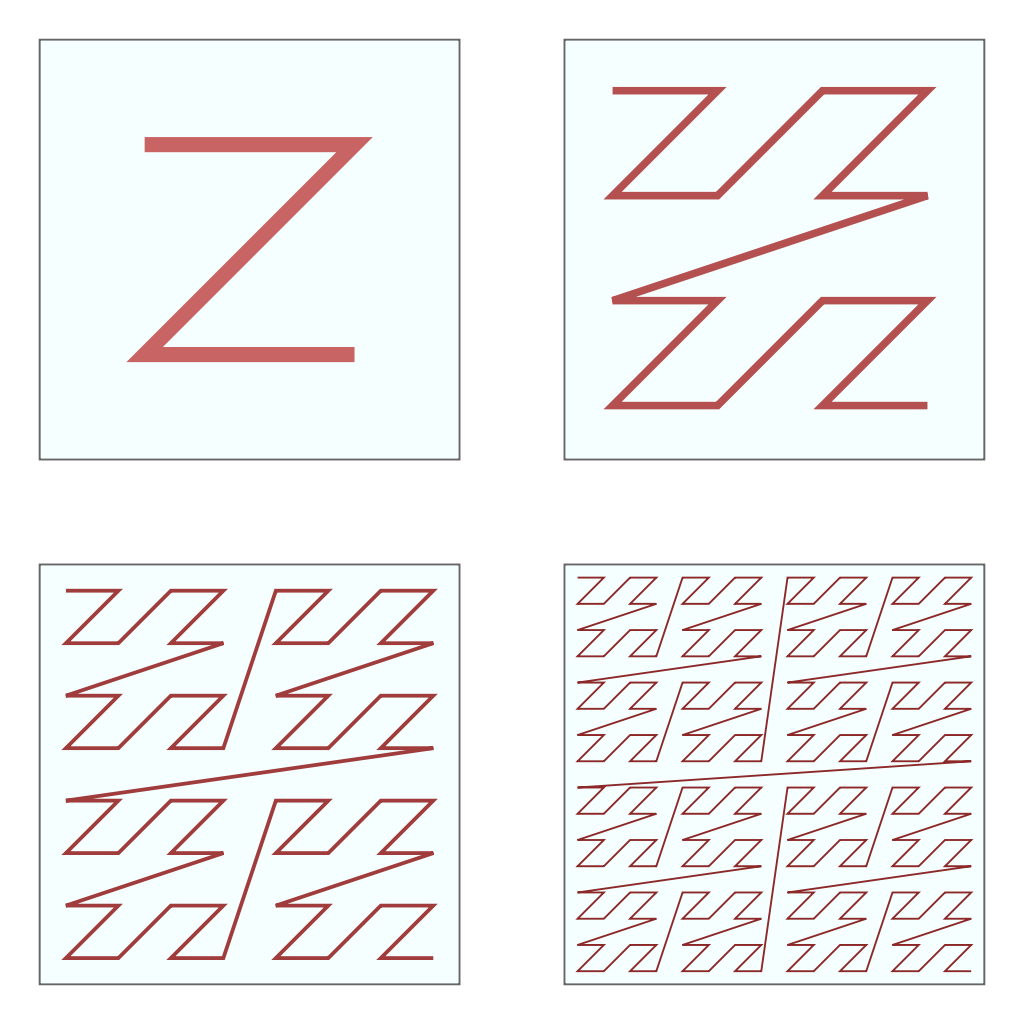
\includegraphics[scale=.2]{morton_order.png}}
\caption{Z-layout}
\label{fig}
\end{figure}

\subsection{Parallel Matrix Multiplication}
We just parallelized the outermost loop of the simple matrix multiplication algorithm
described in section 2.1.

\subsection{Parallel Strassen Algorithm}

\section{Experiments}
	
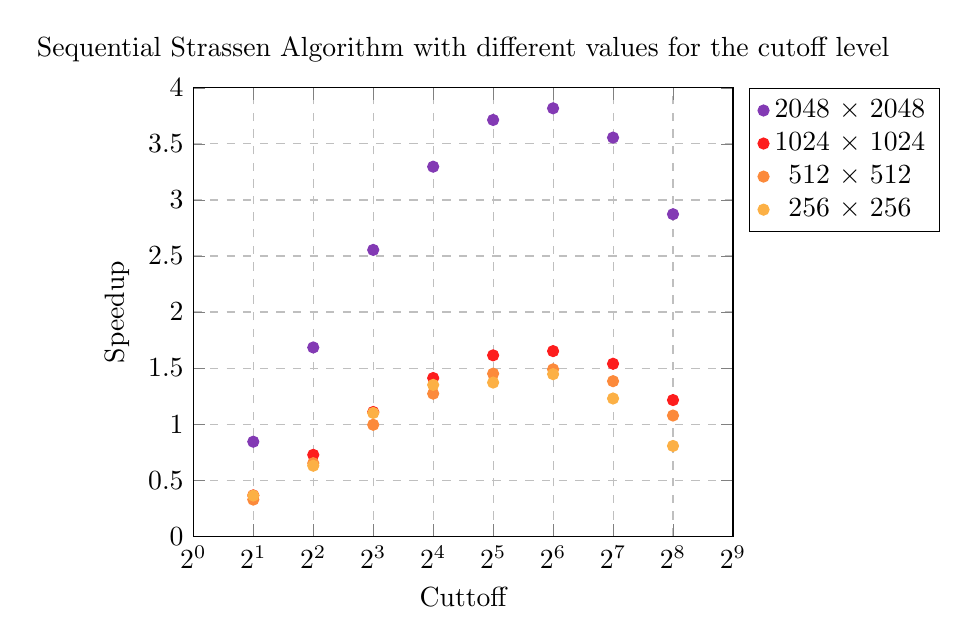
\begin{tikzpicture}
\begin{axis}[
    title={Sequential Strassen Algorithm with different values for the cutoff level},
    xlabel={Cuttoff},
    ylabel={Speedup},
    xmin=1, xmax=512,
    ymin=0, ymax=4,
    xtick={0,1,2,4,8,16,32,64,128,256,512},
    ytick={0, 0.5, 1, 1.5, 2, 2.5, 3, 3.5, 4},
	xmode=log,
    log basis x={2},
    legend pos=outer north east,
    xmajorgrids=true,
    ymajorgrids=true,
    grid style=dashed,
]

 \addplot[
    color=gradient1,
    mark=*,
    only marks,
    ]
    coordinates {
    % running time of normal sequential: 22.729855
     (2, 0.8429769135)(4, 1.6839890956)(8, 2.5542670016)(16, 3.2968112104)(32, 3.7138089218)(64, 3.8177959134)(128, 3.556450524)(256, 2.8727691346)
    };

 \addplot[
    color=gradient2,
    mark=*,
    only marks,
    ]
    coordinates {
    % running time of normal sequential: 1.397876
     (2, 0.3643141647)(4, 0.7259570318)(8, 1.1082371204)(16, 1.4111962817)(32, 1.613661235)(64, 1.6513519133)(128, 1.5385655071)(256, 1.2147025062)
    };

\addplot[
    color=gradient3,
    mark=*,
    only marks,
    ]
    coordinates {
    % running time of normal sequential: 0.177942
     (2, 0.3265631968)(4, 0.6516255667)(8, 0.9941393701)(16, 1.2717773521)(32, 1.4503146089)(64, 1.4886806659)(128, 1.3831910825)(256, 1.0765442556)
    };
    
    \addplot[
    color=gradient4,
    mark=*,
    only marks,
    ]
    coordinates {
    % running time of normal sequential: 0.032513
     (2, 0.3625648174)(4, 0.6287808463)(8, 1.0997496956)(16, 1.350095507)(32, 1.3708154145)(64, 1.4456647399)(128, 1.2285623673)(256, 0.8052157115)
    };
    \legend{2048 $\times$ 2048, 1024 $\times$ 1024, 512 $\times$ 512, 256 $\times$ 256}
    
    
    
\end{axis}
\end{tikzpicture}

\section{Conclusion}

\printbibliography

\end{document}